%!TEX root = ../GLUTthesis.tex
\section{附录1} % 无章节编号
在 MATLAB 上实现用伪谱方法求解非线性 Schr\"odinger 方程
\begin{lstlisting}[language=Matlab,
  morekeywords={},
  emph={fft, ifft, ode45},
  caption={伪谱方法求解三阶孤子}
  ]
    %% 参数设置
    sgn = -1;
    T_max = 10; N_t = 256; 
    t = 2*T_max/N_t*[-N_t/2:N_t/2-1];
    omega = (pi/T_max)*[0:N_t/2-1 -N_t/2:-1].';
    Z = 4; h = 0.2;
    z = 0:h:Z;

    %% 初始条件
    u = 3*sech(t); ut = fft(u);

    %% ODE求解
    [z, UT] = ode45('NLSE', z, ut, [], sgn, omega);
    U = ifft(UT, [], 2);

    %% 可视化
    figure
    waterfall(t, z, abs(U));
    xlabel('时间T/T_0'), ylabel('传输距离z/L_D'), zlabel('强度')
    figure
    waterfall(fftshift(omega)./(2.*pi), z, abs(fftshift(UT, 2)));
    xlabel('频率(\nu-\nu_0)T_0'), ylabel('传输距离z/L_D'), zlabel('频谱强度')
\end{lstlisting}
其中,调用 ode45 时需要自定义表达常微分方程的函数
\begin{lstlisting}[language=Matlab,
  morekeywords={},
  emph={fft, ifft},
  caption={}
  ]
    function dut = NLSE(z, ut, dummy, sgn, omega)
    %NLSE 函数表示被求解的 ODE 方程
    %   dut = i*sgn/2*(omega^2)*ut+i*F[|u|^2*u]
    u = ifft(ut);
    dut = sgn*(i/2)*(omega.^2).*ut+i*fft((abs(u).^2).*u);
    end
\end{lstlisting}

\newpage
\section{附录2}
在 MATLAB 上实现用分步 Fourier 方法求解非线性 Schr\"odinger 方程
\begin{lstlisting}[language=Matlab,
  morekeywords={},
  emph={fft, ifft, ode45},
  caption={分步 Fourier 方法求解三阶孤子}
  ]
    %% 参数设置
    beta_2 = -1; N = 1;
    T_max = 10; N_t = 512;
    Z = 4; h = 0.01;
    t = 2*T_max/N_t*[-N_t/2:N_t/2-1];
    omega = (pi/T_max).*[0:N_t/2-1 -N_t/2:-1];
    z = 0:h:Z;
    
    %% 色散项和非线性项
    D = exp(1i/2*beta_2*omega.^2*h);
    NL = 1i*N^2*h;
    
    %% 初始条件
    u = 3*sech(t);
    U = []; UT = [];
    U(1,:) = u; UT(1,:) = fftshift(fft(u));
    
    %% 分步 Fourier 求解 1/2N->D->1/2N
    u = u.*exp(abs(u).^2.*NL/2);
    for n = 2:length(z)
        ut = fft(u).*D;
        u = ifft(ut);
        u = u.*exp(abs(u).^2.*NL);
        u_r = u.*exp(-abs(u).^2.*NL/2);
        U(n,:) = u_r;
        UT(n,:) = fftshift(fft((u_r)));
    end

    %% 可视化
    figure
    waterfall(t, z, abs(U));
    xlabel('时间T/T_0'), ylabel('传输距离z/L_D'), zlabel('强度')
    figure
    waterfall(fftshift(omega)./(2.*pi), z, abs(UT));
    xlabel('频率(\nu-\nu_0)T_0'), ylabel('传输距离z/L_D'), zlabel('频谱强度')    
\end{lstlisting}

\newpage
%%%%%%%%%%%%%%%%%%%%%%%%%%%%%%%%%
\section{附录3}
在 MATLAB 上实现用有限差分法求解非线性 Schr\"odinger 方程
\begin{lstlisting}[language=Matlab,
  morekeywords={},
  emph={spdiags,inv},
  caption={有限差分法求解三阶孤子}
  ]
  %% 参数设置
  Z_max = 4; T_max = 10;
  dz = 0.0001; dt = 0.002; lambda = dz/dt^2/2;
  z = [0:dz:Z_max]; t = [-T_max:dt:T_max];
  [T, Z] = meshgrid(t, z);
  N_t = length(t); N_z = length(z);
  
  %% 差分矩阵
  e = ones(N_t, 1);
  A = spdiags([lambda/2*e, (1i-lambda)*e, lambda/2*e], [-1, 0, 1], N_t, N_t);
  A(1, N_t) = lambda/2; A(N_t, 1) = lambda/2;
  B = spdiags([-lambda/2*e, (1i+lambda)*e, -lambda/2*e], [-1, 0, 1], N_t, N_t);
  B(1, N_t) = -lambda/2; B(N_t, 1) = -lambda/2;
  A_i = inv(A);
  
  %% 边界条件
  u = 3*sech(t)'; U(1,:) = u';
  
  %% 差分求解
  for m = 2:N_z
      F = B*u-dz*abs(u).^2.*u;
      u = A_i*F;
      U(m,:) = u';
  end
  
  %% 可视化
  figure
  surf(T, Z, abs(U));
  xlabel('时间T/T_0'), ylabel('传输距离z/L_D'), zlabel('强度')
\end{lstlisting}

\newpage
%%%%%%%%%%%%%%%%%%%%%%%%%%%%%%%%%
\section{附录4}
\begin{table}[htbp]
  \centering
  \caption*{伪谱方法的数值实验结果(耗时记录)}
  \begin{tabular}{lcccccc}
    \toprule 
      $\Delta \xi$ & $N_\tau$ & 基阶孤子/s & 二阶孤子/s & 三阶孤子/s & 四阶孤子/s & 五阶孤子/s \\
    \midrule  
      0.1 & 256 & 0.913524 & 0.867968 & 1.087755 & 结果发散 & 结果发散 \\
      0.05 & 256 & 0.8847945 & 0.904476 & 1.126649 & 结果发散 & 结果发散 \\
      0.03 & 256 & 0.906814 & 0.887762 & 1.105801 & 结果发散 & 结果发散 \\
      0,01 & 256 & 0.961330 & 0.959687 & 1.207335 & 结果发散 & 结果发散 \\
      0.005 & 256 & 1.032782 & 1.017613 & 1.255176 & 结果发散 & 结果发散 \\
      0.003 & 256 & 1.128874 & 1.152278 & 1.403453 & 结果发散 & 结果发散 \\
      0.001 & 256 & 1.605832 & 1.594857 & 1.800561 & 结果发散 & 结果发散 \\
      0.1 & 512 & 4.150410 & 4.064225 & 4.060273 & 4.303629 & 5.136246 \\
      0.05 & 512 & 4.163852 & 4.063956 & 4.088162 & 4.283738 & 5.169811 \\
      0.03 & 512 & 4.083730 & 4.160560 & 4.200042 & 4.375078 & 5.205791 \\
      0.01 & 512 & 4.245213 & 4.231423 & 4.255282 & 4.445187 & 5.340950 \\
      0.005 & 512 & 4.390212 & 4.398500 & 4.402081 & 4.643569 & 5.505080 \\
      0.003 & 512 & 4.787179 & 4.706263 & 4.750699 & 4.907478 & 5.813890 \\
      0.001 & 512 & 5.457064 & 5.476309 & 5.466284 & 5.646329 & 6.594705 \\
    \bottomrule
    \end{tabular}
\end{table}

\begin{table}[tbp]
  \centering
  \caption*{分步 Fourier 方法的数值实验结果(耗时记录)}
  \begin{tabular}{lcccccc}
    \toprule 
      $\Delta \xi$ & $N_\tau$ & 基阶孤子/s & 二阶孤子/s & 三阶孤子/s & 四阶孤子/s & 五阶孤子/s \\
    \midrule
      0.1 & 256 & 0.011991 & 0.011326 & 结果发散 & 结果发散 & 结果发散 \\
      0.05 & 256 & 0.012258 & 0.012525 & 结果发散 & 结果发散 & 结果发散 \\
      0.03 & 256 & 0.019958 & 0.015117 & 结果发散 & 结果发散 & 结果发散 \\
      0.01 & 256 & 0.047944 & 0.048051 & 0.040772 & 0.046679 & 结果发散 \\
      0.005 & 256 & 0.098894 & 0.101310 & 0.102865 & 0.101067 & 结果发散 \\
      0.003 & 256 & 0.438257 & 0.431412 & 0.416631 & 结果发散 & 结果发散 \\
      0.001 & 256 & 4.911769 & 4.917287 & 4.916656 & 4.927861 & 结果发散 \\
      0.1 & 512 & 0.010518 & 0.010189 & 结果发散 & 结果发散 & 结果发散 \\
      0.05 & 512 & 0.013548 & 0.015026 & 结果发散 & 结果发散 & 结果发散 \\
      0.03 & 512 & 0.020160 & 0.019286 & 结果发散 & 结果发散 & 结果发散 \\
      0.01 & 512 & 0.066089 & 0.059894 & 0.058442 & 结果发散 & 结果发散 \\
      0.005 & 512 & 0.362146 & 0.371222 & 0.359213 & 结果发散 & 结果发散 \\
      0.003 & 512 & 1.137290 & 1.163925 & 1.134111 & 1.150079 & 1.142337 \\
      0.001 & 512 & 9.897807 & 9.908339 & 9.984559 & 9.904616 & 9.893836 \\
    \bottomrule
    \end{tabular}
\end{table}

\newpage
\section*{MATLAB 编程要点}
\subsection*{ODE 求解器的调用}
在 MATLAB 中调用 ODE 求解器通常需要一个调用指令 odesolver 和一个函数定义文件 odefun.m。{\bfseries odesolver 的调用语法为}
$$
\mathrm{[X,U]=odesolver(odefun, xspan, u0, options, parameter1, parameter2, \ldots)}
$$
\begin{enumerate}[label=(\arabic*)]
  \item “odesolver”是所调用求解器的函数名称,可以是 ode45、ode23、ode113、ode15s、ode23s、ode23t、ode23tb 和 ode15i 中的一个。
  \item “odefun”是定义常微分方程组 $u'_i=f_i(x,u_1,u_2,\ldots,u_n)$ 的函数句柄,可以是 odefun.m 文件定义的函数,也可以是“@”标记的匿名函数。
  \item “xspan”是表示常微分方程组自变量 $x$ 取值范围的向量 $[x_0,x_1,x_2,\ldots,x_n]$。
  \item “u0”是代表常微分方程组初始条件的向量 $u_i(x_0)$。
  \item “options”是一个改变 odesolver 默认参数设置的结构体,是一个可选参数。若不改变默认参数设置,可将其设置为空。
  \item “parameter1, parameter2,\ldots”是传递给 odefun 的参数,是可选项。
  \item “[X,U]”保存计算结果。向量 X 就是自变量的离散取值 $[x_0,x_1,x_2,\ldots,x_n]$,矩阵 U 就是所求常微分方程组的数值解。
\end{enumerate}

{\bfseries odefun 函数的定义需要与 odesolver 的调用形式相对应}
$$
\mathrm{function\; du\; =\; odefun(x, u, dummy,  parameter1, parameter2, \ldots)}
$$
\begin{enumerate}[label=(\arabic*)]
  \item “odefun”为函数名,函数文件名必须与其相同。
  \item “x”为自变量。
  \item “u”是常微分方程组的函数值 $u_i(x)$,是一个矩阵。
  \item “dummy”是一个占位符,无实际意义。
  \item “parameter1, parameter2, \ldots”用于接收传递来的参数。
  \item “du”为函数输出结果的变量名。
\end{enumerate}

\subsection*{fftshift 操作}
由于 FFT 算法本身的原因,fft 函数的输出结果在频域上是颠倒的
$$
0\;,2\pi/T_0\;,4\pi/T_0,\ldots,(2N-4)\pi/T_0\;,(2N-2)\pi/T_0\;,-2N\pi/T_0\;,-(2N-2)\pi/T_0,\ldots,-4\pi/T_0\;,-2\pi/T_0
$$
因此需要 fftshift 函数调整 fft 输出序列的顺序。但是在分步 Fourier 方法(伪谱方法)求解问题时,不需要每次运算都调整频谱顺序,只需将最后一步运算的频谱结果调整即可(频率序列首先需要人为颠倒,可视化时再调整回来)。

\subsection*{spdiags 函数创建带状矩阵}
$$
\mathrm{A\; =\; spdiags(B,d,m,n)}
$$
通过获取 B 的列并沿 d 指定的对角线放置它们,来创建一个 m×n 带状矩阵。

\subsection*{可视化模板}
\begin{multicols}{2}
  \begin{lstlisting}[language=Matlab,
  morekeywords={},
  emph={waterfall, view, colormap},
  caption={}
  ]
    %% 瀑布图可视化
    figure
    waterfall(t, z, abs(U))
    view(-45,45)
    xlabel('时间 T/T_0'),
    ylabel('传输距离 z/L_D'),
    zlabel('强度'),
    axis([-10 10 0 inf 0 inf]),
    colormap([0 0 0]); 
  \end{lstlisting}
  \begin{figure}[H]
    \centering
    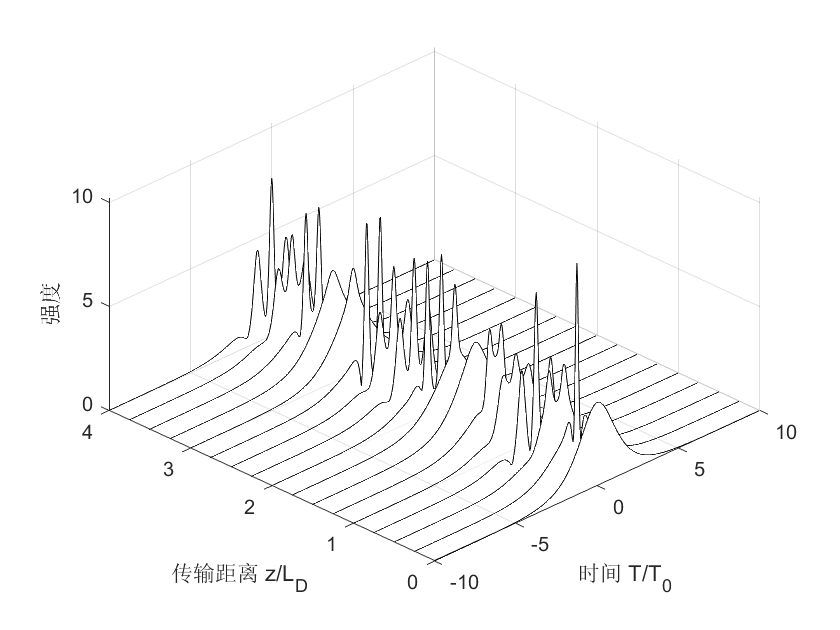
\includegraphics[width=0.35\textwidth]{瀑布图可视化.png}
    % \caption{瀑布图可视化}
  \end{figure}
\end{multicols}

\begin{multicols}{2}
  \begin{lstlisting}[language=Matlab,
  morekeywords={},
  emph={meshgrid, surf, shading, view, colormap},
  caption={}
  ]
    %% 曲面图可视化
    [T, Z] = meshgrid(t, z);
    figure
    surf(T, Z, abs(U))
    xlabel('时间 T/T_0'),
    ylabel('传输距离 z/L_D'),
    zlabel('强度'),
    view(-20,70)
    axis([-10 10 0 inf 0 inf]),
    shading interp
    colormap(gca, 'jet');
  \end{lstlisting}
  \begin{figure}[H]
    \centering
    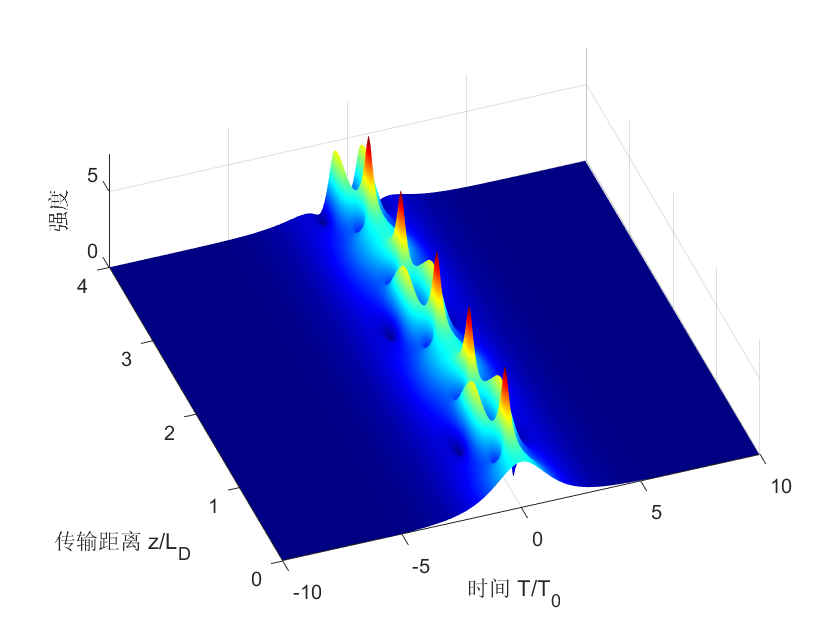
\includegraphics[width=0.35\textwidth]{曲面图可视化.png}
    % \caption{曲面图可视化}
  \end{figure}
\end{multicols}
